\chapter{雨天车道线数据集构建与增强}
\label{cha:dataset_construction}

\section{引言}
\label{sec:intro_3}

高质量标注数据集是深度学习模型获得稳定性能的重要前提。对于雨天车道线检测任务而言，训练数据的质量与多样性尤为关键，因为模型在真实恶劣天气中的表现，很大程度上取决于训练样本是否覆盖了主要干扰场景。然而，现有主流车道线检测数据集（如 TuSimple\cite{tusimple}、CULane\cite{pan2018spatial}）虽然规模较大、标注规范，但采集场景仍以晴天或良好光照条件为主，雨天样本占比较低，对降雨强度和路面积水状态的区分也不够细致。这种数据层面的缺口，使得基于通用数据集训练的模型在雨天场景中容易出现明显性能退化，即域偏移（Domain Shift）问题\cite{porav2019}。

为从数据层面对上述问题作出回应，本章围绕雨天车道线专用数据集 RainLane 的构建展开。内容主要包括四个方面：分析雨天干扰因素对车道线视觉特征的影响，说明真实场景数据采集与标注流程，介绍针对雨天特性设计的数据增强策略，并对数据集的整体构成与使用方式进行说明。结合目前已完成的整理工作，RainLane 已按 CULane 的目录结构组织，可直接适配 CLRNet 的训练与测试流程；原始有效标注样本共 6017 张，经增强后样本规模扩展至 24068 张。


\section{雨天干扰因素对车道线视觉特征的影响分析}
\label{sec:rain_impact_analysis}

\subsection{雨天环境的物理干扰机制}

雨天对车载视觉系统的干扰源于多种物理现象的耦合作用，主要可归纳为以下三类：

\textbf{（1）雨滴遮挡与模糊效应}

悬浮或附着于摄像头镜头表面的雨滴，会对穿透光线产生折射与散射作用，在图像中形成局部模糊斑点和光晕区域。降雨过程中，镜头前方运动的雨丝（Rain Streak）在有限曝光时间内形成运动模糊，其典型表现为方向性线状噪声，在图像中呈现出与车道线方向相近的倾斜条纹，极易干扰特征提取模块对车道线边缘的响应。设雨滴在图像坐标系中的位置为 $(x_0, y_0)$，其遮挡半径为 $r$，则受遮挡图像区域 $\Omega_r$ 可近似表示为：
\begin{equation}
	\Omega_r = \{(x, y) \mid (x - x_0)^2 + (y - y_0)^2 \leq r^2\}
\end{equation}
对于 $\Omega_r$ 内的像素点，其观测灰度值 $I_\text{obs}$ 可建模为原始信号与雨滴透射函数的混合：
\begin{equation}
	I_\text{obs}(x, y) = \alpha \cdot I_\text{rain}(x, y) + (1 - \alpha) \cdot I_\text{scene}(x, y), \quad (x, y) \in \Omega_r
	\label{eq:raindrop_model}
\end{equation}
其中 $\alpha \in [0,1]$ 为雨滴的不透明度系数，$I_\text{rain}$ 为雨滴折射所呈现的背景光亮度，$I_\text{scene}$ 为无遮挡条件下的场景真实灰度值。实际中，多个雨滴往往同时存在，其遮挡区域相互叠加，导致大面积图像信息缺失。


\textbf{（2）路面水膜与镜面反射效应}

降雨在路面形成连续或不连续的水膜层，显著改变了路面的光学特性。干燥柏油路面具有漫反射特性（Lambert表面），其双向反射率（BRDF）分布较为均匀；而水膜覆盖后，路面转变为近镜面反射体，其表面亮度 $L_\text{wet}$ 受入射光方向与视角的强烈影响，遵循菲涅耳反射定律\cite{fresnel}：
\begin{equation}
	R_F(\theta) = \frac{1}{2} \left[ \frac{\sin^2(\theta_i - \theta_t)}{\sin^2(\theta_i + \theta_t)} + \frac{\tan^2(\theta_i - \theta_t)}{\tan^2(\theta_i + \theta_t)} \right]
	\label{eq:fresnel}
\end{equation}
其中 $\theta_i$ 为入射角，$\theta_t$ 为折射角，二者满足斯涅尔定律。水膜的镜面反射将天空、路灯、对向车灯等强光源的像投影于路面，形成大面积高亮反光区域，其亮度值往往远超车道线标志本身，使得后续检测算法难以有效区分车道线特征与水膜反射噪声。


\textbf{（3）降雨大气散射与对比度退化}

雨天大气中悬浮的大量细小水滴形成散射介质，光线在传播过程中被多次散射，导致场景的视觉对比度整体下降。根据Koschmieder大气散射模型，退化图像 $I(x,y)$ 与无退化理想图像 $J(x,y)$ 之间满足：
\begin{equation}
	I(x, y) = J(x, y) \cdot t(x, y) + A \cdot (1 - t(x, y))
	\label{eq:koschmieder}
\end{equation}
其中 $A$ 为大气光强度，$t(x,y)$ 为介质透射率，其随场景深度 $d(x,y)$ 指数衰减：$t(x,y) = e^{-\beta d(x,y)}$，$\beta$ 为大气散射系数。对于中大雨场景，$\beta$ 显著增大，导致远处车道线的对比度大幅降低，信噪比恶化，极大增加了检测难度。

\subsection{雨天车道线视觉特征的任务化退化分析}

为说明雨天干扰对车道线检测性能的影响，本文从以下三个与检测任务直接相关的特征维度进行分析：

\textbf{（1）对比度退化}：可采用 Michelson 对比度指标 $C = (L_\text{max} - L_\text{min}) / (L_\text{max} + L_\text{min})$ 衡量车道线区域相对于路面背景的亮度差异。随着降雨强度增大和路面积水增多，车道线与背景之间的亮度差通常明显缩小，远处车道线的可辨识性下降更为突出。

\textbf{（2）边缘响应强度}：可借助 Canny 或 Sobel 等算子的响应情况观察车道线边缘的梯度特征。雨天条件下，雨纹噪声会引入大量伪边缘，同时水膜反射使路面亮度趋于均匀，导致车道线真实边缘的梯度响应幅值相对降低，信号噪声比明显下滑。

\textbf{（3）局部遮挡与结构断裂}：当雨滴附着镜头或前车溅水遮挡视野时，车道线会出现局部缺失甚至连续断裂。这类退化并不一定改变整幅图像的整体亮度分布，但会直接破坏检测模型赖以判断车道线走向的连续性信息。

\subsection{雨天干扰对主流检测算法的影响说明}

结合当前训练与测试过程中观察到的现象，可以发现主流检测算法在雨天场景中的失效大多集中在三类情况：其一，水膜反射形成与车道线相近的高亮条带，容易引发误检；其二，雨滴遮挡导致车道线局部断裂，模型难以保持连续预测；其三，雨纹、模糊与低对比度共同作用时，行方向定位会出现明显漂移。上述现象说明，雨天条件下的失效并非单一噪声所致，而是多类退化叠加后的结果，这也为后续在特征层引入抗干扰模块提供了直接动机。


\section{数据标注与质量控制}
\label{sec:data_annotation}

\subsection{真实雨天数据的采集方案}

本研究依托课题组已有的车载采集平台，制定了系统化的雨天场景数据采集方案。采集设备采用车载前视摄像头，安装于驾驶舱内前挡风玻璃后方，位置符合 ADAS 常规部署规范。采集过程尽可能覆盖不同降雨强度、不同道路类型以及不同光照条件，以保证后续数据集能够反映真实道路环境中的主要干扰形态。

采集场景遵循多维度覆盖原则，具体涵盖：
\begin{itemize}[leftmargin=2em]
	\item \textbf{降雨强度}：依据中国气象局标准，分别采集小雨（日降水量 $<$ 10 mm）、中雨（10--25 mm）、大雨（$>$ 25 mm）四类场景；
	\item \textbf{时间段}：包含白天（自然光充足）、傍晚（弱光过渡）、夜间（人工照明为主）三类光照条件，以捕捉不同光照与雨天的耦合干扰；
	\item \textbf{道路类型}：涵盖城市主干道（多车道、宽车道）、城市次干道（交叉口密集）、郊区公路（双向双车道）、高速公路（高速行驶、车道标志鲜明）等典型场景；
	\item \textbf{路面状态}：区分刚开始降雨（路面轻微湿润）、持续降雨（路面明显积水）、雨后初晴（路面潮湿反光）三种路面状态，以充分覆盖不同阶段的水膜特性。
\end{itemize}

在原始图像筛选阶段，剔除了曝光过度、剧烈抖动、严重遮挡以及车道线几乎不可辨识的低质量样本，最终形成 6017 张可用于标注与实验的有效图像。随后，按照训练、验证与测试流程对数据进行整理，并在训练阶段配合雨天增强策略扩展样本规模。


\subsection{标注规范设计}

本课题所构建数据集的标注格式与基本规范参照主流公开数据集 CULane\cite{pan2018spatial} 执行，以确保与现有研究基准的兼容性。针对雨天图像中车道线模糊、断裂等特有挑战，在遵循通用标注框架的基础上，制定了以下具体操作细则。

\textbf{(1) 标注粒度与表示形式}：采用实例级多段折线标注方式，每条车道线由一系列有序坐标点表示，作为独立实例处理。标注结果以文本形式存储，每幅图像对应一份标注文本，其中每一行对应一条车道线实例，格式为一系列空格分隔的浮点数坐标对：
\begin{verbatim}
	x_{1} y_{1} x_{2} y_{2} ... x_{n} y_{n}
\end{verbatim}
坐标点沿车道线中心线等距采样，采样间隔约为 10 像素，以在保证标注精度的同时控制标注工作量。

\textbf{(2) 标注范围与规则}：标注范围覆盖图像中清晰可见且可可靠辨识的所有车道线，包括本车道左右边界线及相邻车道边界线。对于因视距限制、严重遮挡或图像边缘截断导致无法连续追踪的部分，标注终止于最后可明确判定的位置。标注过程中不进行超出可见范围的主观推测性延伸。

\textbf{(3) 雨天断点处理策略}：雨天场景中，雨滴遮挡、积水反光等因素易造成车道线局部断裂。本数据集遵循保守标注原则——仅标注清晰、连续可见的车道线段，不对断裂区域进行人为插值补全。若断裂长度导致车道线走向无法可靠判断，则将车道线拆分为独立线段分别记录于同一标注中，由后续检测模型自行学习处理断裂情形。该策略避免了引入标注偏差，保证了数据的客观性与可复现性。

\textbf{(4) 标注工具与流程}：采用LabelMe工具进行辅助标注，标注人员沿车道线中心线逐点标记。完成标注后，通过专用转换程序将中间标注结果批量整理为标准坐标文本格式，并对坐标序列进行等距重采样，以保证数据分布与主流预训练模型输入的一致性。

\begin{figure}[htbp]
	\centering
	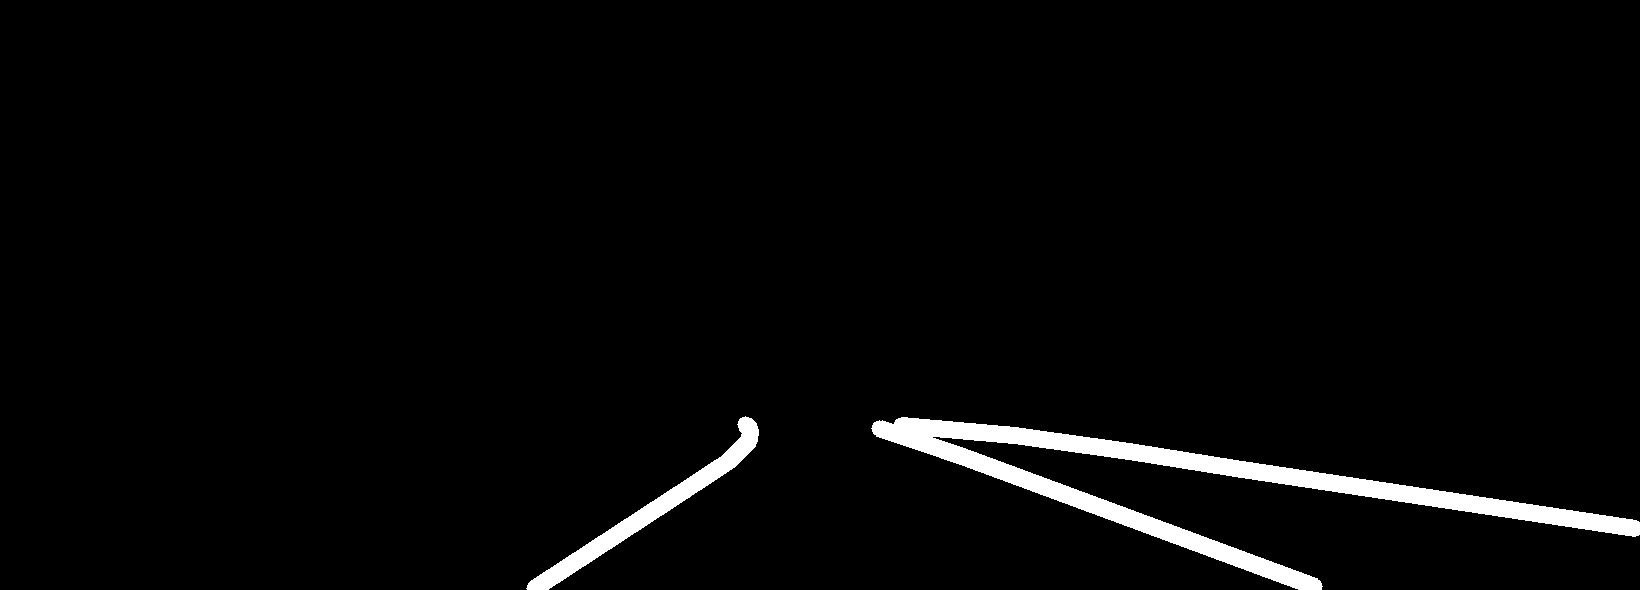
\includegraphics[width=0.8\textwidth]{image/chap03/vis_lane.png}
	\caption{LabelMe标注雨天车道线标注可视化示例}
	\label{fig:labelme-example}
\end{figure}

\subsection{标注质量控制机制}

为保障标注质量，本研究建立了三级质控机制：

\textbf{初级审核}：由经过培训的标注人员完成初始标注后，由另一名标注人员进行交叉复核，重点检查断点续标的合理性与折线关键点的密度是否满足规范要求。

\textbf{一致性检验}：对同一图像进行双人独立标注，计算折线关键点的 Hausdorff 距离；若超过预设阈值，则提交进一步复核，以减少关键点偏移和断点处理不一致带来的标注误差。

\textbf{模型辅助检验}：利用预训练 CLRNet 模型对标注结果进行预检测，将模型检测结果与人工标注进行对比，自动标记差异较大的样本供人工复审，以捕捉可能存在的大面积标注错误。

经三级质控后，最终形成可用于训练、验证与测试的有效标注样本 6017 张，并完成与后续训练流程匹配的数据整理工作。


\section{雨天车道线专用数据集的构建与增强}
\label{sec:dataset_building}

\subsection{数据集整体结构}

本研究构建的雨天车道线专用数据集命名为 RainLane。其整体结构设计主要遵循三项原则：一是尽量覆盖不同降雨强度、道路类型与光照条件的组合，以保证场景多样性；二是控制各类样本数量分布，尽量避免明显失衡；三是保留必要的元数据与场景标签，便于后续进行细粒度划分与复现实验。根据当前统计结果，数据集共包含 6017 张有效标注图像，其中训练集 4208 张、验证集 904 张、测试集 905 张。

表\ref{tab:dataset_split}给出了RainLane数据集的样本分布情况。

\begin{table}[htbp]
	\centering
	\caption{RainLane数据集样本分布统计}
	\label{tab:dataset_split}
	\begin{tabularx}{\textwidth}{@{}YYYYY@{}}
		\toprule
		\textbf{场景类别} & \textbf{训练集} & \textbf{验证集} & \textbf{测试集} & \textbf{合计} \\
		\midrule
		强反光/积水 & 123  & 27  & 27  & 177  \\
		中雨 & 1,546 & 332 & 332 & 2,210 \\
		明显遮挡 & 1,322 & 283 & 284 & 1,889 \\
		小雨 & 482  & 104 & 104 & 690  \\
		大雨/暴雨 & 735  & 158 & 158 & 1,051 \\
		\midrule
		\textbf{合计} & \textbf{4,208} & \textbf{904} & \textbf{905} & \textbf{6,017} \\
		\bottomrule
	\end{tabularx}
\end{table}


数据集按照7:1.5:1.5的比例划分为训练集、验证集与测试集，其中测试集严格独立，不参与任何超参数调优过程，用于最终性能的无偏评估。在数据组织上，训练样本与测试样本分别独立存放，并为每张图像配备对应的折线标注文本，以保证后续训练、验证和测试流程的一致性。


\subsection{数据增强策略设计}

受限于实际数据采集条件，特定极端场景（如强暴雨夜间高速公路）的真实样本数量有限，单纯依靠真实数据难以满足深度学习模型的训练需求。为此，本研究构建了系统化的雨天数据增强流水线，从以下几个层次对数据集进行扩充：

\textbf{（1）通用几何与光度增强}

在保持车道线标注有效性的前提下，对图像施加以下通用增强操作：
\begin{itemize}[leftmargin=2em]
	\item 随机水平翻转（翻转概率50\%，同步翻转标注坐标）；
	\item 随机亮度与对比度扰动（亮度因子 $\beta \in [-30, 30]$，对比度因子 $\alpha \in [0.7, 1.3]$）；
	\item 随机色调（Hue）与饱和度（Saturation）扰动（$\Delta H \in [-10, 10]$，$\Delta S \in [0.8, 1.2]$）；
	\item 随机高斯模糊（核大小 $\in \{3, 5\}$，$\sigma \in [0.5, 2.0]$），模拟摄像头散焦；在图~\ref{fig:gaussian_blur_comparison}中，右图为施加核大小 $15 \times 15$、$17 \times 17$、$19 \times 19$、$\sigma \in [4.0, 8.0]$ 的高斯模糊后的结果，用于模拟雨天摄像头散焦效应。
	\item 随机仿射变换（小角度旋转 $\theta \in [-5^\circ, 5^\circ]$（中雨及以上强度），平移范围 $\pm 5\%$），提升模型对轻微相机抖动的鲁棒性。
\end{itemize}

\begin{figure}[htbp]
	\centering
	\begin{subfigure}[b]{0.48\textwidth}
		\centering
		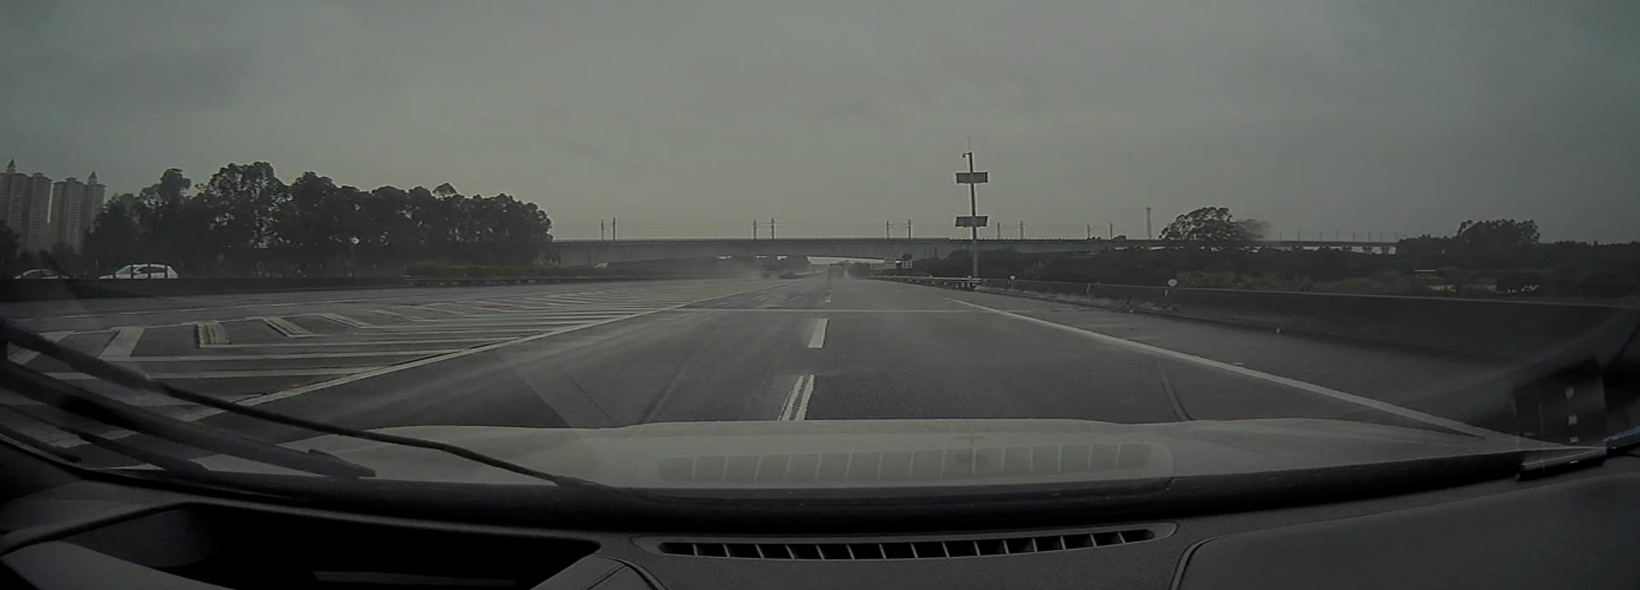
\includegraphics[width=\textwidth]{image/chap03/s4_2427000_原图.jpg}
		\caption{原始图像}
		\label{fig:blur_original}
	\end{subfigure}
	\hfill
	\begin{subfigure}[b]{0.48\textwidth}
		\centering
		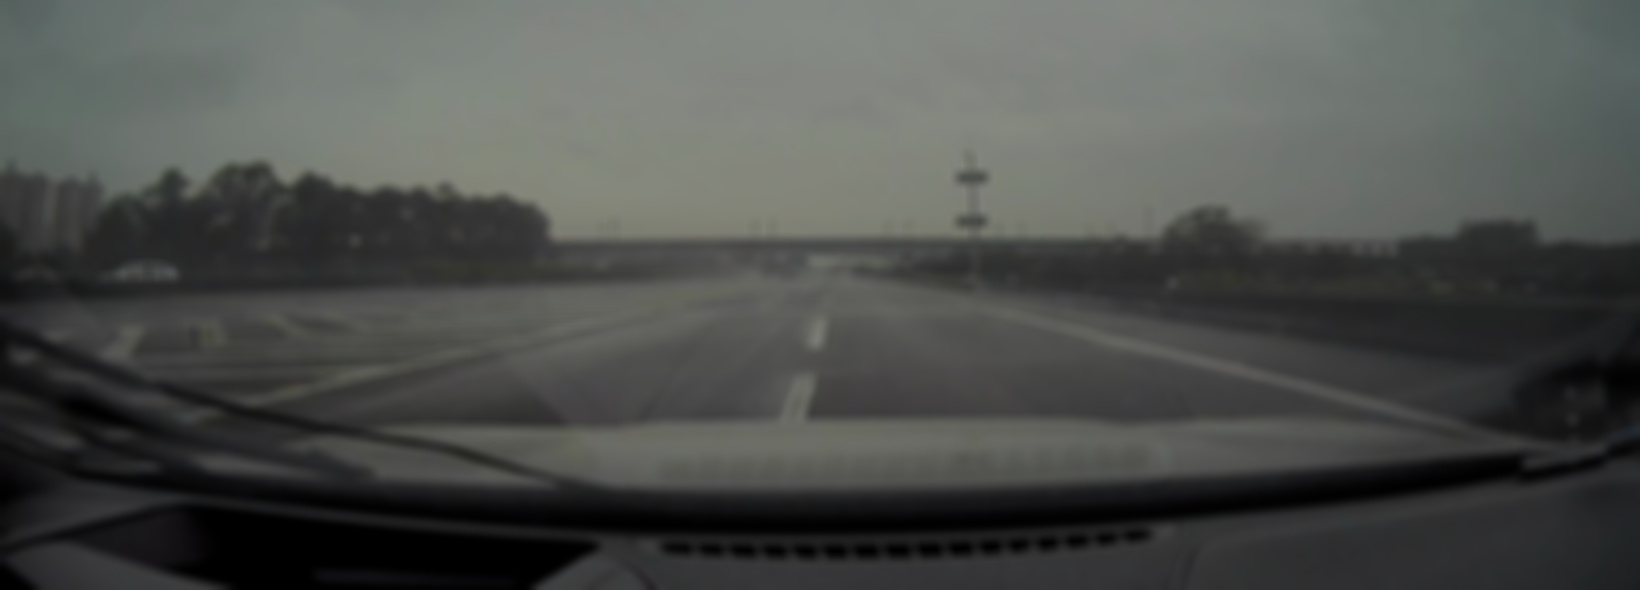
\includegraphics[width=\textwidth]{image/chap03/s4_2427000_高斯模糊.jpg}
		\caption{高斯模糊后}
		\label{fig:blur_result}
	\end{subfigure}
	\caption{随机高斯模糊增强效果}
	\label{fig:gaussian_blur_comparison}
\end{figure}


\textbf{（2）雨纹合成增强}

雨纹（Rain Streak）合成是针对雨天场景最为关键的数据增强手段。本研究采用的雨纹合成方法与本文实际使用的增强流程保持一致，可生成具有真实感的雨纹噪声\cite{zhang2018}。合成流程如下：

首先，生成随机雨滴线段集合。每根雨纹建模为具有一定宽度和长度的线段，其主导方向角 $\theta_\text{main}$ 在 $[-8^\circ, 8^\circ]$ 内随机选取，并叠加 $\pm (2^\circ \sim 6^\circ)$ 的随机角度扰动以增加自然感。雨纹长度 $L \in [20, 100]$ 像素（实际代码中通过动态选取最小长度20--40像素、最大长度50--100像素实现），宽度 $w \in [1, 3]$ 像素，亮度值 $I_s \in [180, 255]$，以模拟不同粗细、明暗程度的雨丝。

其次，将雨纹层与原始图像进行Alpha混合，合成退化图像 $I_\text{syn}$：
\begin{equation}
	I_\text{syn}(x, y) = (1 - \lambda) \cdot I_\text{orig}(x, y) + \lambda \cdot S(x, y)
	\label{eq:rain_synthesis}
\end{equation}
其中 $S(x,y)$ 为雨纹层图像，$\lambda$ 为混合系数，控制雨纹的视觉强度。根据增强强度等级 $\gamma$ 的不同，雨纹数量范围与混合强度设置如下：
\begin{itemize}
	\item $\gamma = 1$（小雨）：雨纹数量 $N \in [200, 800]$，混合强度 $\lambda = 0.3$；
	\item $\gamma = 2$（中雨）：雨纹数量 $N \in [500, 1500]$，混合强度 $\lambda = 0.5$；
	\item $\gamma = 3$（大雨/暴雨）：雨纹数量 $N \in [1000, 2000]$，混合强度 $\lambda = 0.7$。
\end{itemize}

此外，通过施加核大小为3或5的高斯模糊使雨纹边缘更柔和，提升合成真实感。

\begin{figure}[htbp]
	\centering
	\begin{subfigure}[b]{0.48\textwidth}
		\centering
		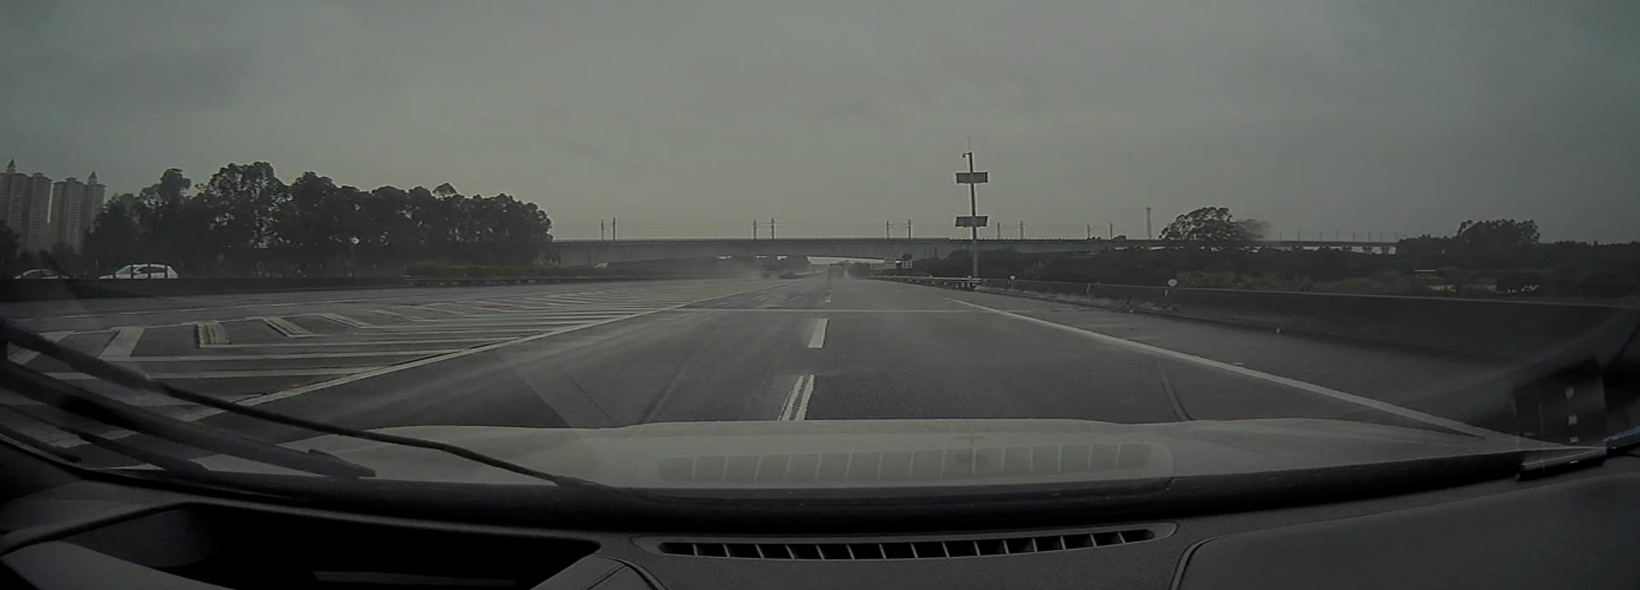
\includegraphics[width=\textwidth]{image/chap03/s4_2427000_原图.jpg}
		\caption{原图}
		\label{fig:aug_grid_1}
	\end{subfigure}
	\hfill
	\begin{subfigure}[b]{0.48\textwidth}
		\centering
		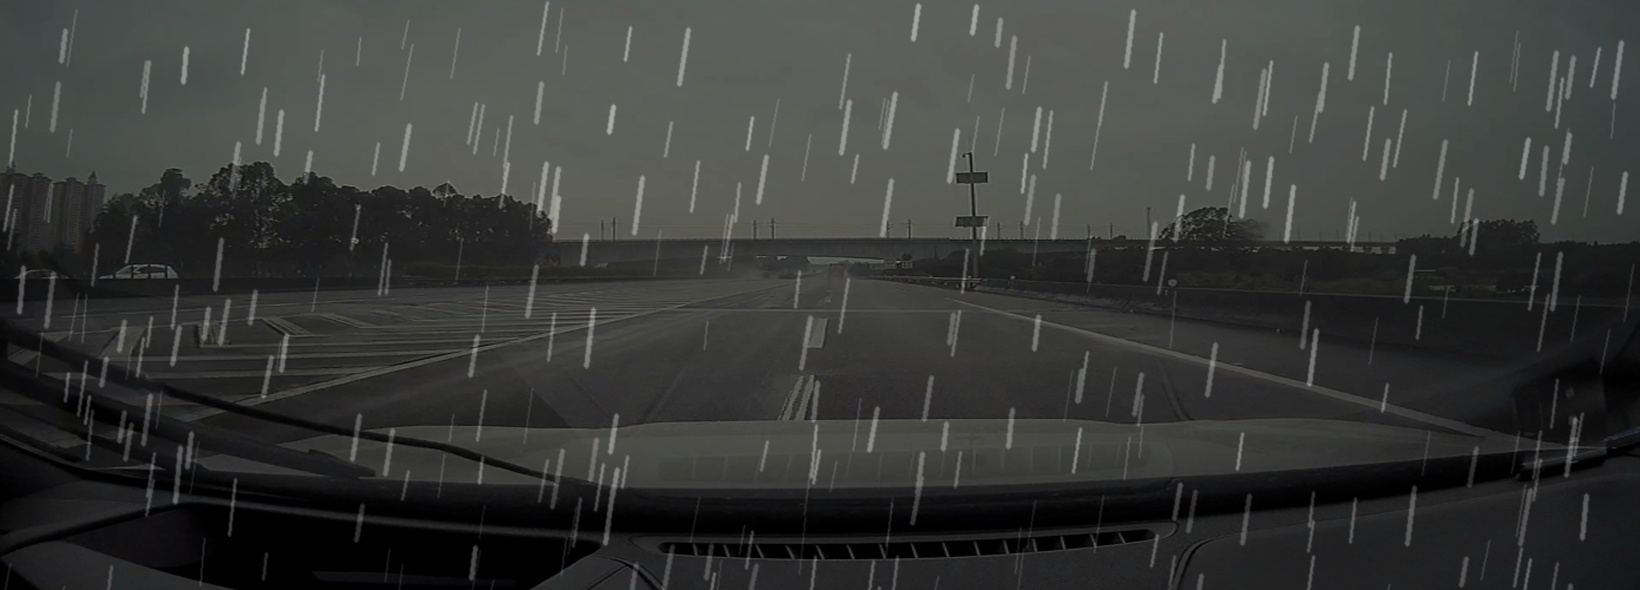
\includegraphics[width=\textwidth]{image/chap03/s4_2427000_小雨.jpg}
		\caption{小雨}
		\label{fig:aug_grid_2}
	\end{subfigure}
	
	\vspace{0.5em}
	
	\begin{subfigure}[b]{0.48\textwidth}
		\centering
		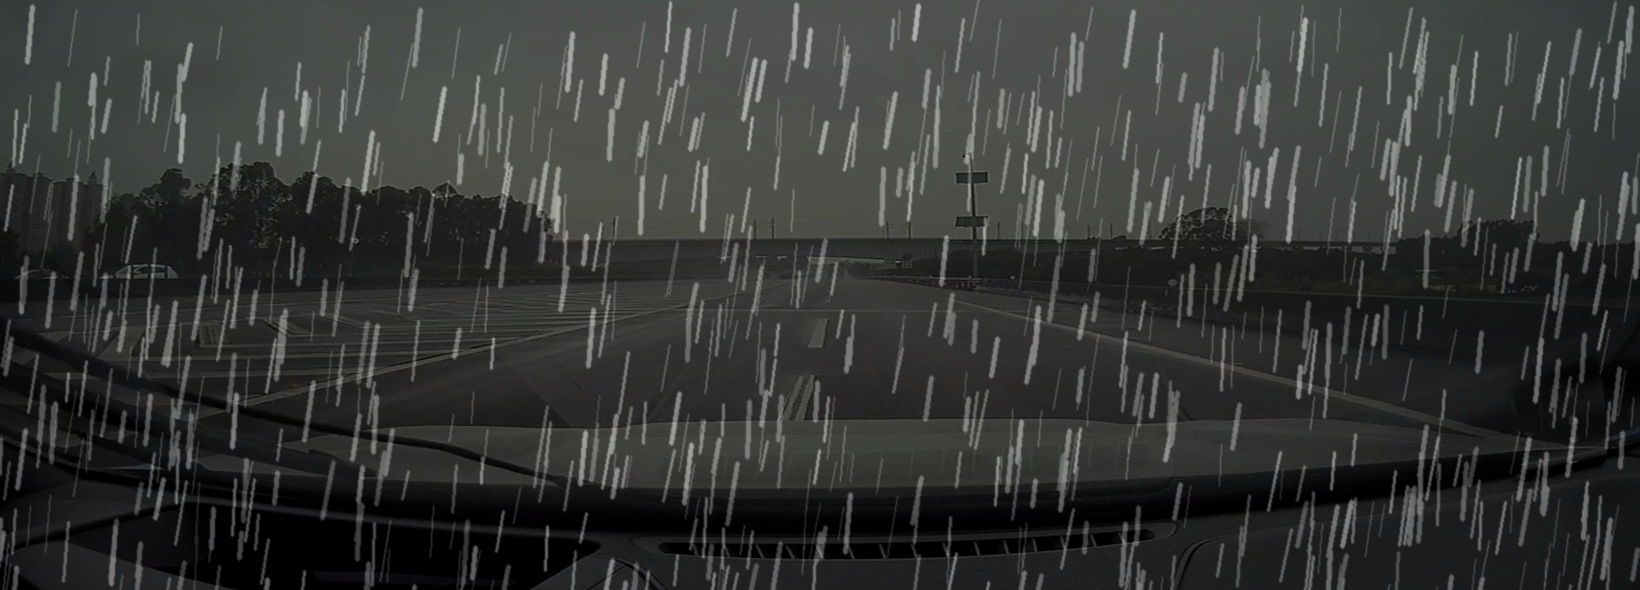
\includegraphics[width=\textwidth]{image/chap03/s4_2427000_中雨.jpg}
		\caption{中雨}
		\label{fig:aug_grid_3}
	\end{subfigure}
	\hfill
	\begin{subfigure}[b]{0.48\textwidth}
		\centering
		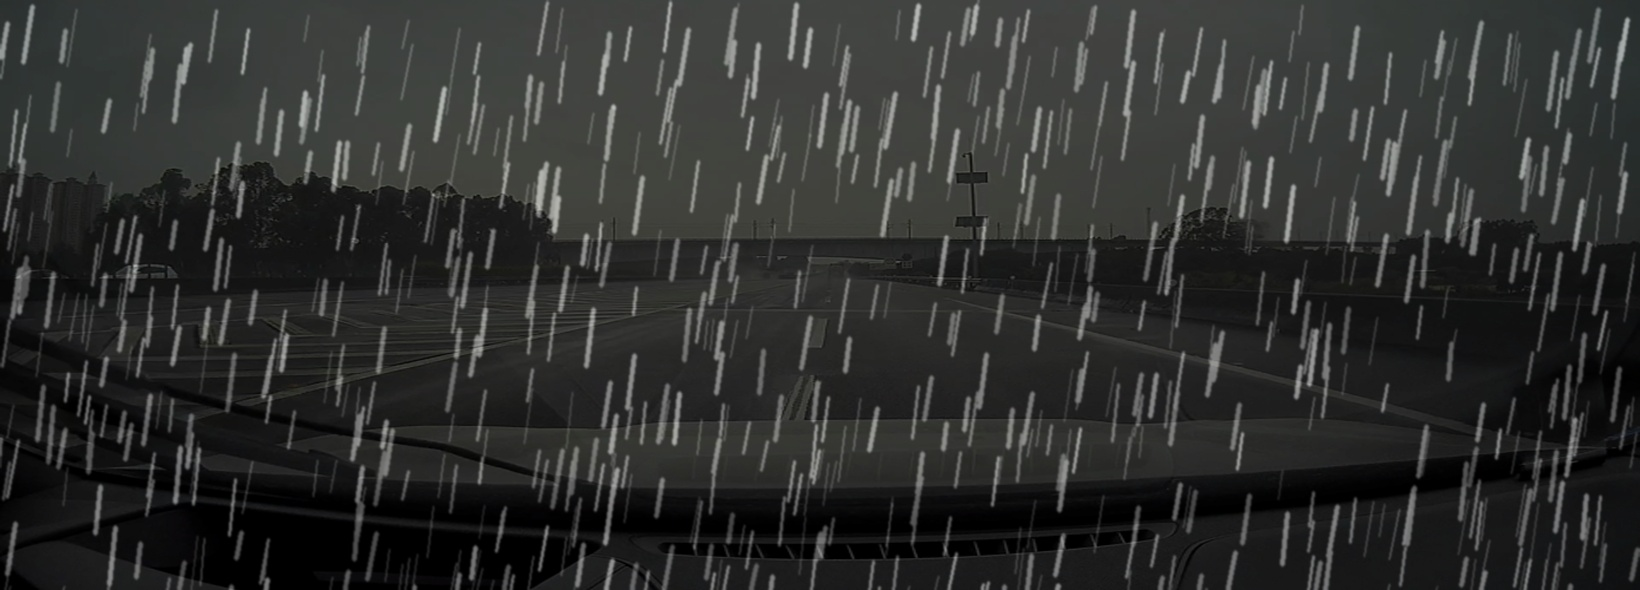
\includegraphics[width=\textwidth]{image/chap03/s4_2427000_大雨.jpg}
		\caption{大雨}
		\label{fig:aug_grid_4}
	\end{subfigure}
	
	\caption{不同强度雨纹合成效果对比}
	\label{fig:data_augmentation_2x2}
\end{figure}

\textbf{（3）水膜反射模拟增强}

路面水膜反射是雨天场景中最难以通过简单合成还原的干扰因素之一。本研究采用以下近似方案进行模拟：

识别图像中路面区域（利用深度估计先验或语义分割先验获取粗略路面掩码 $M_\text{road}$，实际代码中简化为图像下半部分区域），在路面区域内随机选取1--8个圆形反射区域（半径30--100像素），将区域亮度提升30\%--60\%，模拟水膜镜面反射效果：
\begin{equation}
	I_\text{reflect}(x, y) = I_\text{orig}(x, y) \cdot (1 + \mu), \quad (x,y) \in R_k
	\label{eq:reflection_aug}
\end{equation}
其中 $\mu \in [0.3, 0.6]$ 控制反射强度，$R_k$ 为第 $k$ 个反射区域。该方法虽为近似，但可有效模拟路面反光导致对比度降低的视觉效果，提升模型对水膜反射噪声的鲁棒性。

\begin{figure}[htbp]
	\centering
	\begin{subfigure}[b]{0.48\textwidth}
		\centering
		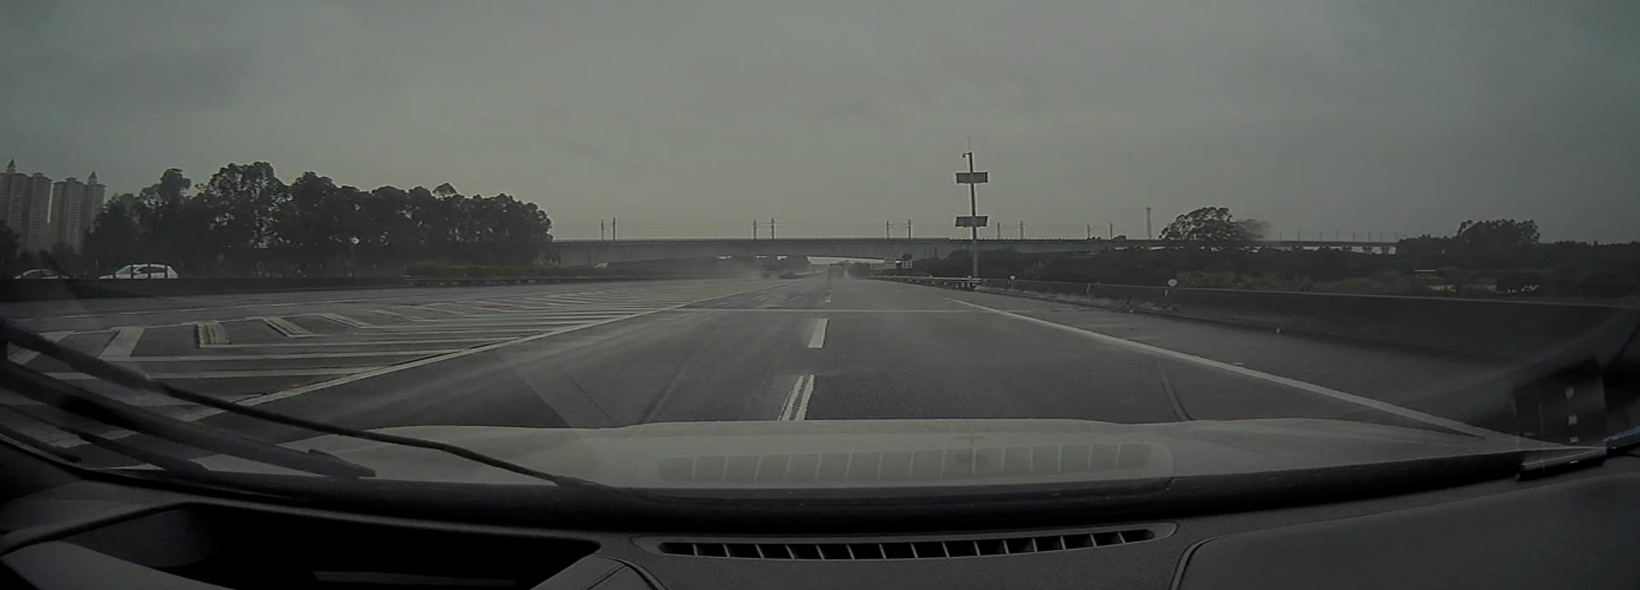
\includegraphics[width=\textwidth]{image/chap03/s4_2427000_原图.jpg}
		\caption{原始图像}
		\label{fig:reflection_original}
	\end{subfigure}
	\hfill
	\begin{subfigure}[b]{0.48\textwidth}
		\centering
		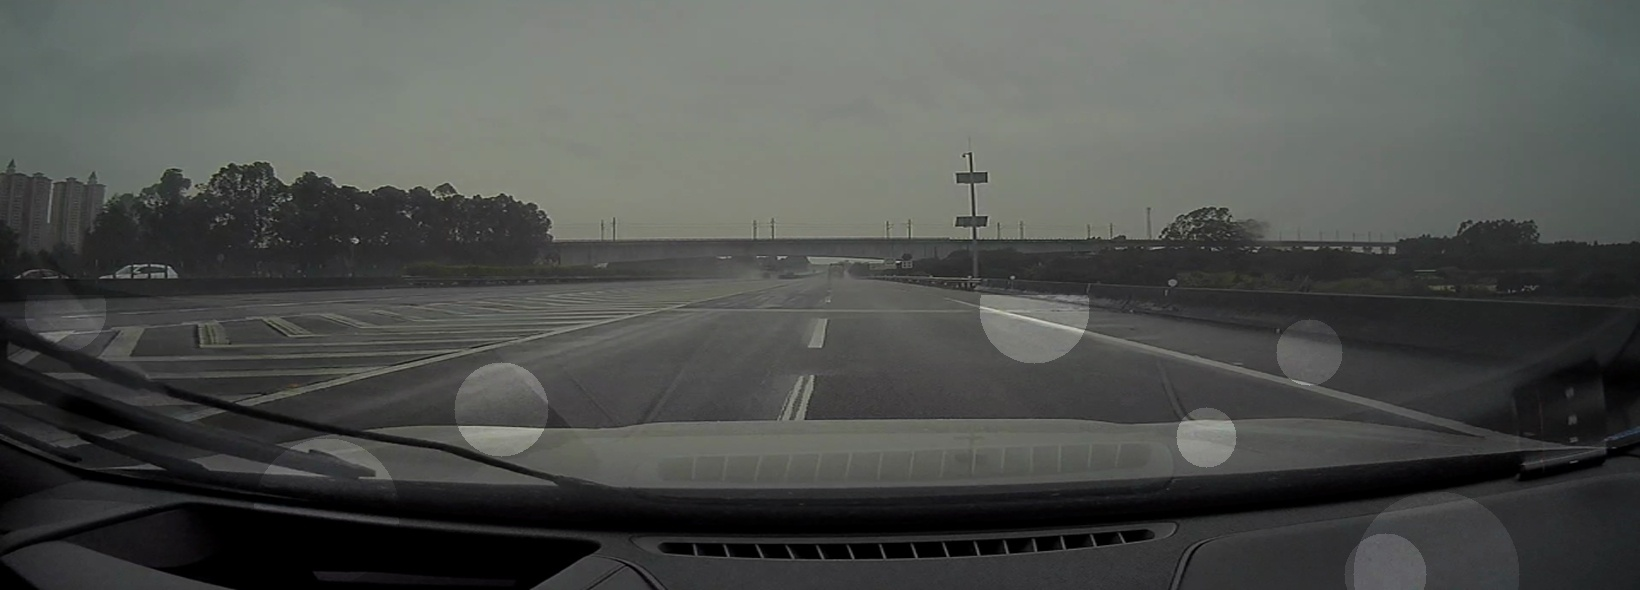
\includegraphics[width=\textwidth]{image/chap03/s4_2427000_重度水膜反射.jpg}
		\caption{水膜反射模拟后}
		\label{fig:reflection_result}
	\end{subfigure}
	\caption{水膜反射模拟增强效果}
	\label{fig:water_reflection_comparison}
\end{figure}

\textbf{（4）CutOut遮挡增强}

为模拟雨滴附着镜头导致的局部信息缺失，采用CutOut\cite{devries2017cutout}策略在图像随机位置遮挡若干矩形区域，强迫模型利用上下文信息推断被遮挡位置的车道线走向，提升模型对局部遮挡的容忍度。参数设置随强度等级调整：
\begin{itemize}
	\item $\gamma = 1$：遮挡数量 $n \in [2, 5]$，矩形尺寸 $[40, 60]$ 像素；
	\item $\gamma = 2$：遮挡数量 $n \in [3, 8]$，矩形尺寸 $[60, 80]$ 像素；
	\item $\gamma = 3$：遮挡数量 $n \in [5, 12]$，矩形尺寸 $[80, 100]$ 像素。
\end{itemize}
遮挡区域填充为该区域原始像素均值，避免引入人为强边缘。图~\ref{fig:cutout_comparison_2x2}中，左上为原始图像，其余三幅分别展示不同增强强度等级下的随机矩形遮挡效果。遮挡区域填充为局部均值，用于模拟雨滴附着镜头导致的局部信息缺失。

\begin{figure}[htbp]
	\centering
	% 第一行：原图 + γ=1
	\begin{subfigure}[b]{0.48\textwidth}
		\centering
		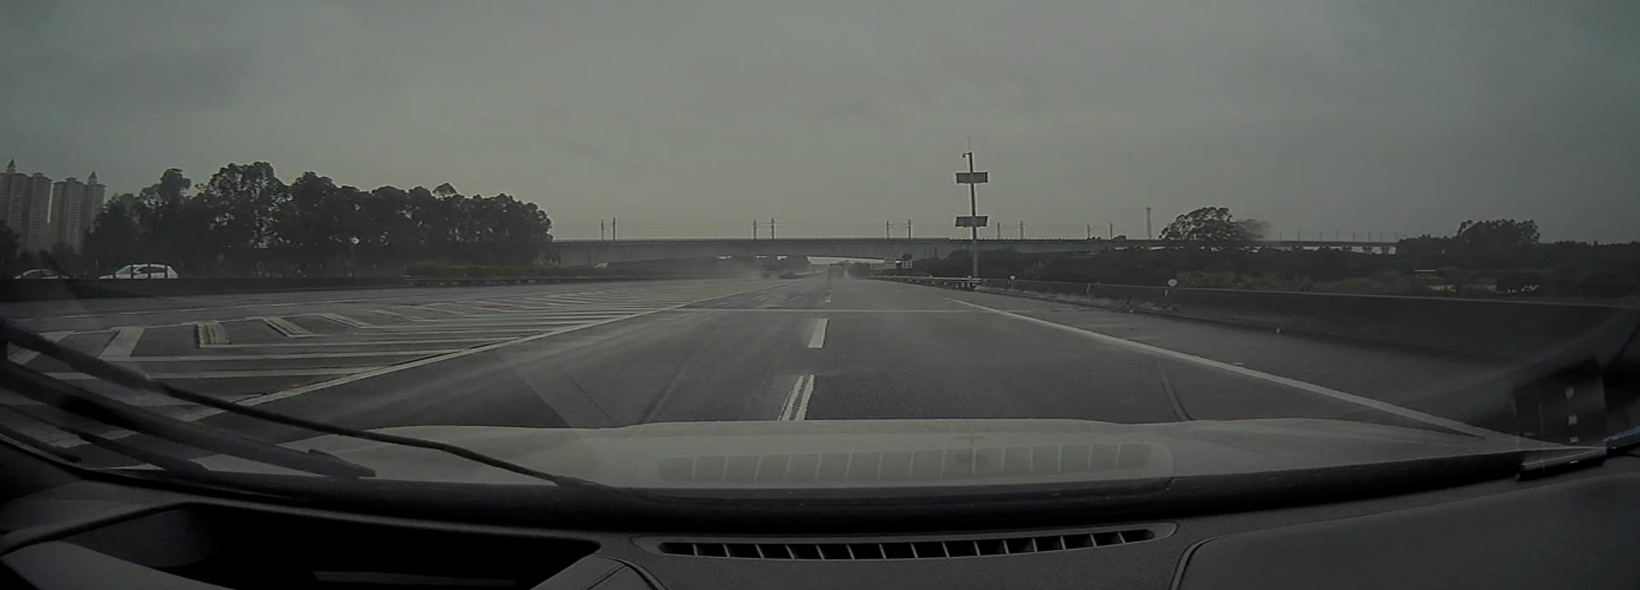
\includegraphics[width=\textwidth]{image/chap03/s4_2427000_原图.jpg}
		\caption{原始图像}
		\label{fig:cutout_original}
	\end{subfigure}
	\hfill
	\begin{subfigure}[b]{0.48\textwidth}
		\centering
		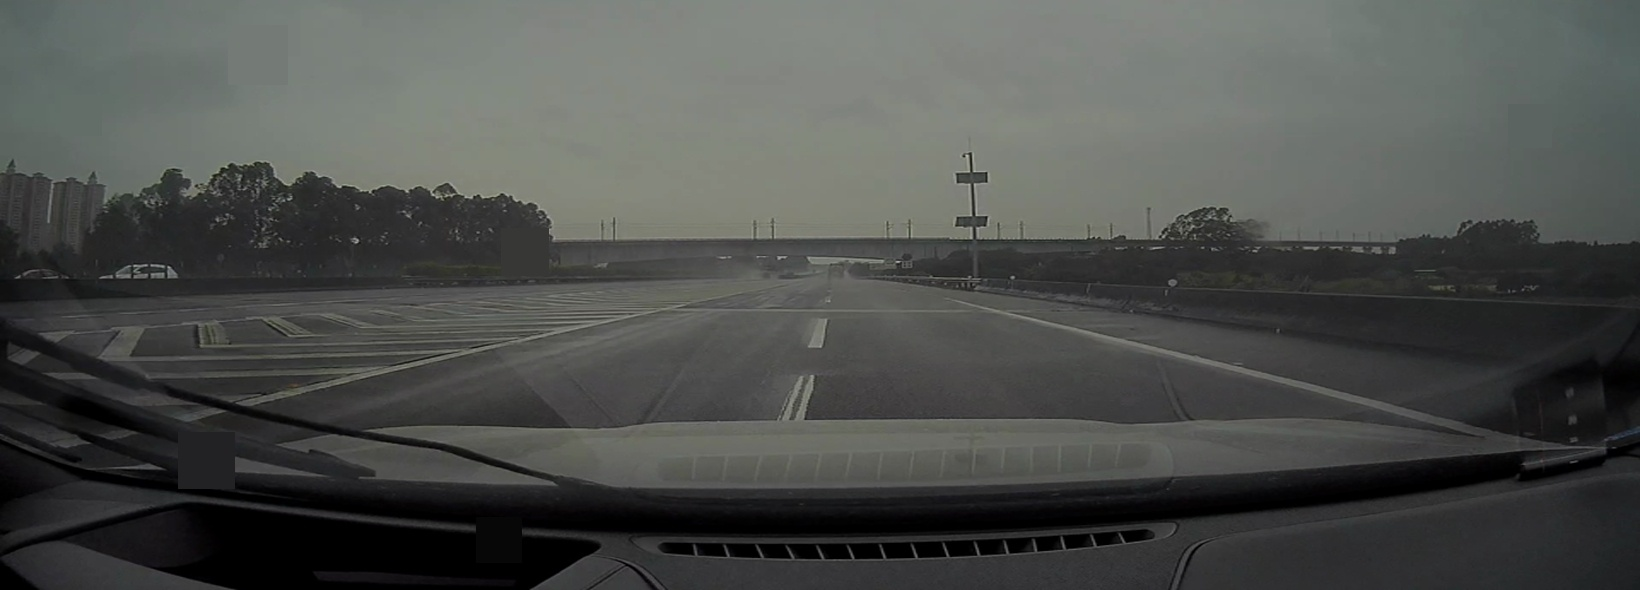
\includegraphics[width=\textwidth]{image/chap03/s4_2427000_轻度遮挡.jpg}
		\caption{$\gamma = 1$（$n \in [2,5]$，尺寸 $[40,60]$）}
		\label{fig:cutout_gamma1}
	\end{subfigure}
	
	\vspace{0.5em}
	
	% 第二行：γ=2 + γ=3
	\begin{subfigure}[b]{0.48\textwidth}
		\centering
		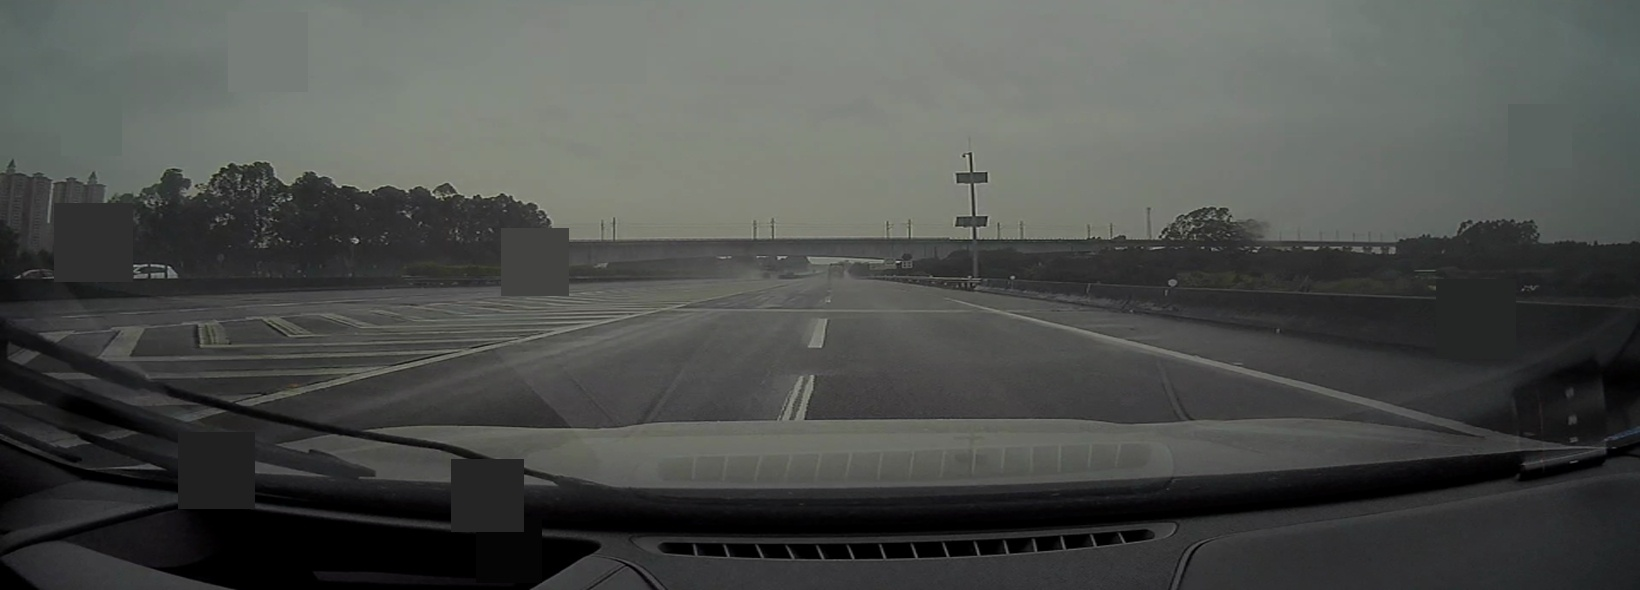
\includegraphics[width=\textwidth]{image/chap03/s4_2427000_中度遮挡.jpg}
		\caption{$\gamma = 2$（$n \in [3,8]$，尺寸 $[60,80]$）}
		\label{fig:cutout_gamma2}
	\end{subfigure}
	\hfill
	\begin{subfigure}[b]{0.48\textwidth}
		\centering
		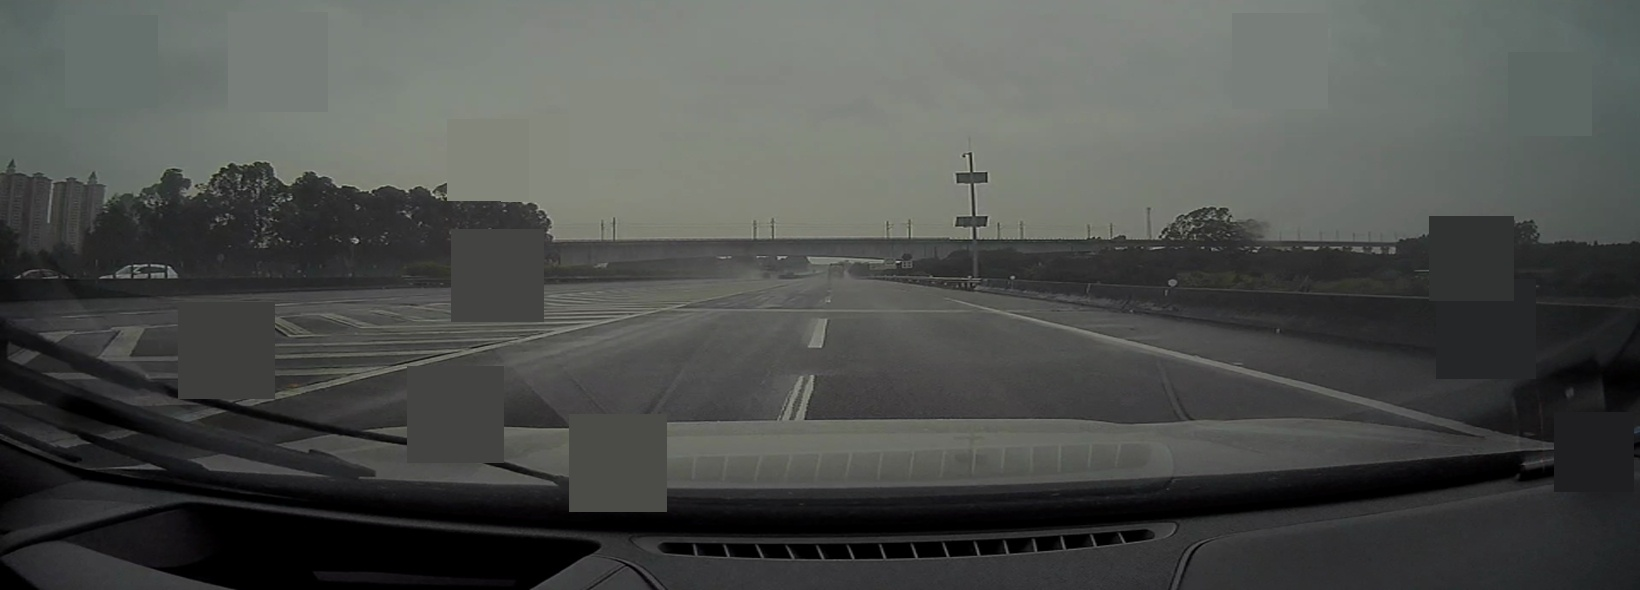
\includegraphics[width=\textwidth]{image/chap03/s4_2427000_重度遮挡.jpg}
		\caption{$\gamma = 3$（$n \in [5,12]$，尺寸 $[80,100]$）}
		\label{fig:cutout_gamma3}
	\end{subfigure}
	
	\caption{CutOut遮挡增强效果对比}
	\label{fig:cutout_comparison_2x2}
\end{figure}

\subsection{增强流水线的组合策略}

在实际训练过程中，上述增强操作并非彼此独立，而是按照一定概率进行组合，形成完整的数据增强流水线，如算法\ref{alg:aug_pipeline}所示。该流程与本文实际采用的样本增强策略保持一致。

\begin{algorithm}[htbp]
	\caption{雨天车道线数据增强流水线}
	\label{alg:aug_pipeline}
	\SetKwInOut{Input}{输入}
	\SetKwInOut{Output}{输出}
	\Input{原始图像 $I$，对应标注 $L$，增强强度等级 $\gamma \in \{1, 2, 3\}$}
	\Output{增强后图像 $I'$，对应标注 $L'$}
	\BlankLine
	\If{以概率 $p=0.5$}{
		施加随机水平翻转，同步更新标注坐标 $L$\;
	}
	\If{以概率 $p=0.8$}{
		施加随机亮度/对比度/色度扰动（$\beta \in [-30,30]$，$\alpha \in [0.7,1.3]$，饱和度因子 $\in [0.8,1.2]$）\;
	}
	\If{以概率 $p=0.6$}{
		施加高斯模糊，核大小随 $\gamma$ 增大（强度 $\leq 1$ 时核 $\in \{3,5\}$，强度 $\geq 2$ 时核 $\in \{3,5,7\}$）\;
	}
	\If{以概率 $p=0.7$}{
		施加雨纹合成：雨纹数量与混合强度按 $\gamma$ 等级选取（$\gamma=1$: $N \in [200,800]$, $\lambda=0.3$；$\gamma=2$: $N \in [500,1500]$, $\lambda=0.5$；$\gamma=3$: $N \in [1000,2000]$, $\lambda=0.7$）\;
	}
	\If{以概率 $p=0.4$}{
		施加水膜反射模拟：在路面区域生成1--4个圆形高亮反射区\;
	}
	\If{以概率 $p=0.5$}{
		施加CutOut遮挡：遮挡数量与尺寸按 $\gamma$ 等级选取\;
	}
	\If{以概率 $p=0.3$}{
		施加随机仿射变换：旋转范围 $\theta \in [-3^\circ, 3^\circ]$（$\gamma=1$）或 $[-5^\circ, 5^\circ]$（$\gamma \geq 2$），平移范围 $\pm 3\%$（$\gamma=1$）或 $\pm 5\%$（$\gamma \geq 2$）\;
	}
	\Return{$I'$，$L'$}
\end{algorithm}

通过调节增强强度等级 $\gamma$，可以控制合成样本的退化程度，使训练集同时覆盖小雨、中雨及大雨条件下的差异化样本。经该流水线处理后，训练集有效样本数量扩充约 4 倍，达到约 24068 张。


\subsection{数据集有效性说明}

结合目前已完成的数据整理与训练适配工作，RainLane 的有效性主要体现在以下三个方面。

\textbf{（1）场景覆盖具有针对性}：数据集中明确包含小雨、中雨、大雨等不同强度场景，并同时覆盖白天与夜间路况，使其能够直接服务于雨天鲁棒检测这一研究目标，而非仅用于一般道路场景识别。

\textbf{（2）组织形式具有可用性}：数据集已按照 CULane 的目录结构与标注格式进行整理，能够与 CLRNet 的训练、验证和测试流程直接对接，减少后续方法比较中由数据接口差异带来的额外变量。

\textbf{（3）增强策略与真实退化相呼应}：高斯模糊、雨纹合成、水膜反射与局部遮挡等增强方式均对应雨天行车中的典型干扰类型，增强后的样本总数扩展至 24068 张，有助于提升模型对不同退化模式的覆盖能力。

\begin{figure}[htbp]
	\centering
	\begin{subfigure}[b]{0.48\textwidth}
		\centering
		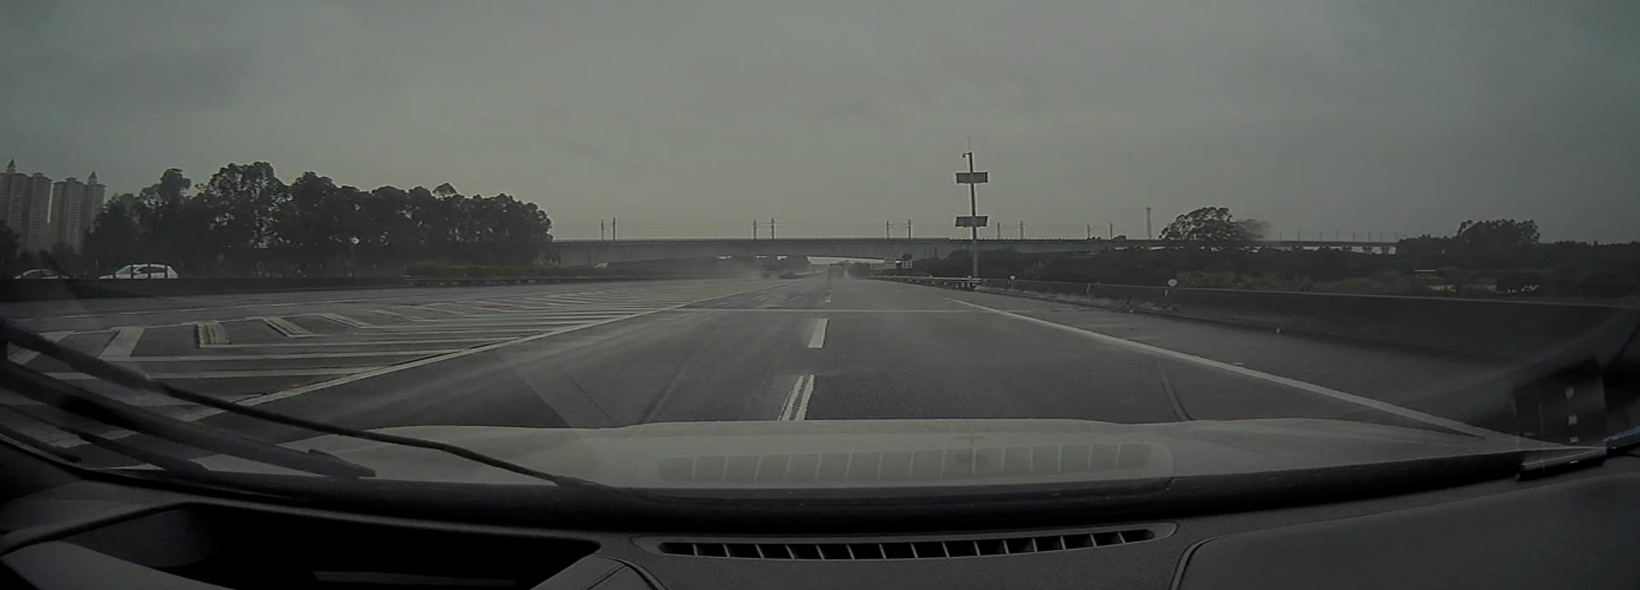
\includegraphics[width=\textwidth]{image/chap03/s4_2427000_原图.jpg}
		\caption{原始场景}
	\end{subfigure}
	\hfill
	\begin{subfigure}[b]{0.48\textwidth}
		\centering
		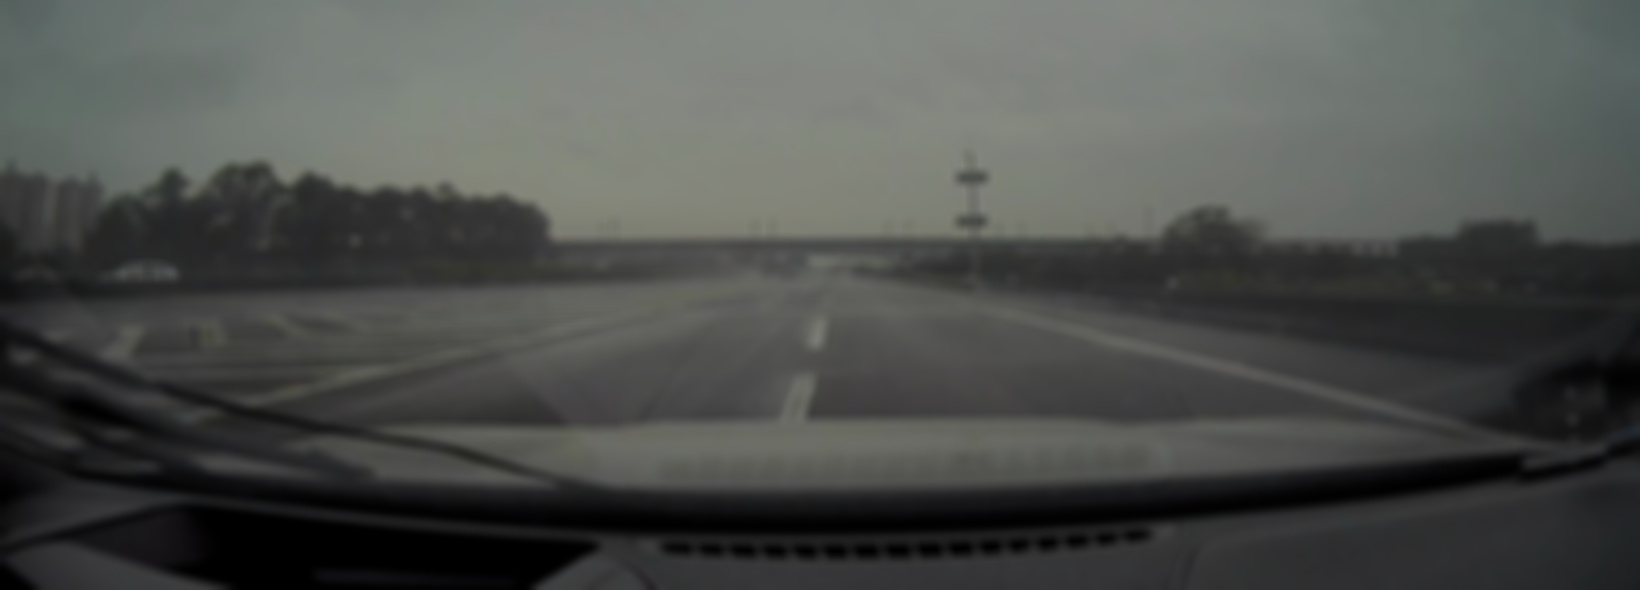
\includegraphics[width=\textwidth]{image/chap03/s4_2427000_高斯模糊.jpg}
		\caption{模糊退化}
	\end{subfigure}

	\vspace{0.5em}

	\begin{subfigure}[b]{0.48\textwidth}
		\centering
		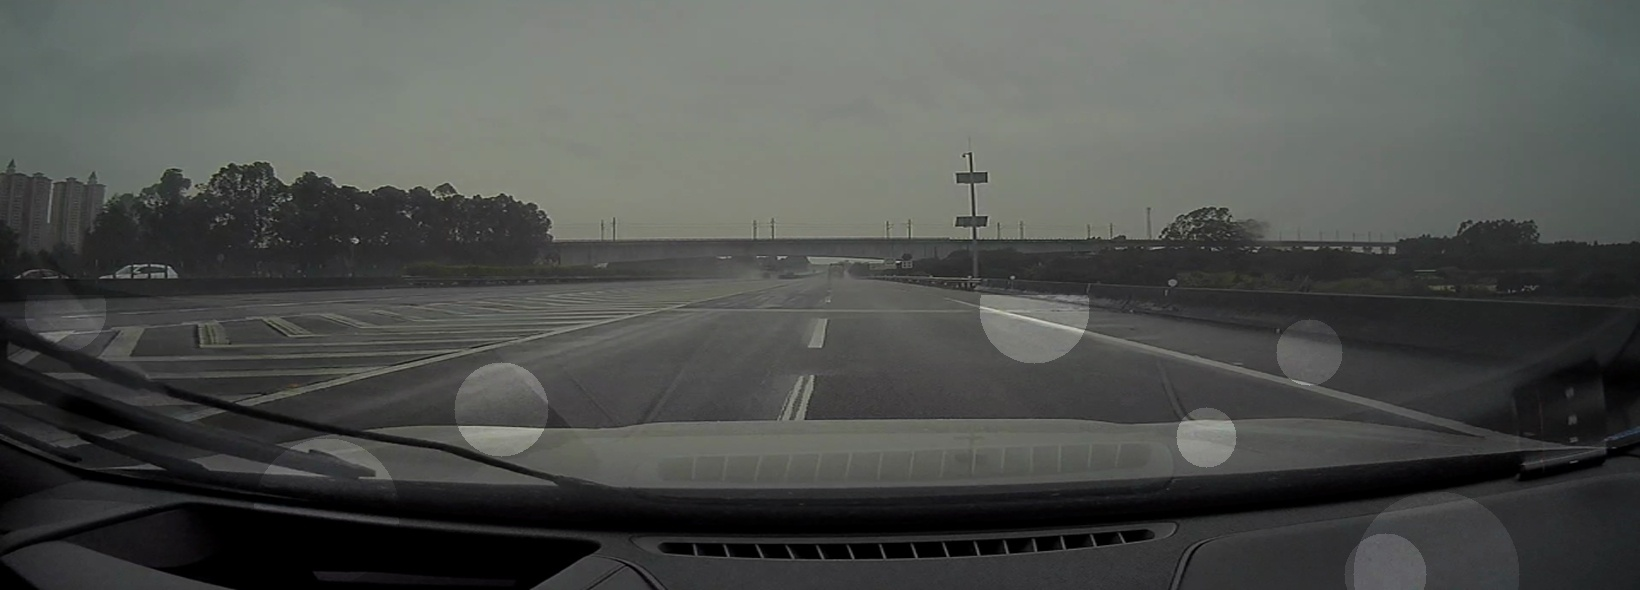
\includegraphics[width=\textwidth]{image/chap03/s4_2427000_重度水膜反射.jpg}
		\caption{水膜反射}
	\end{subfigure}
	\hfill
	\begin{subfigure}[b]{0.48\textwidth}
		\centering
		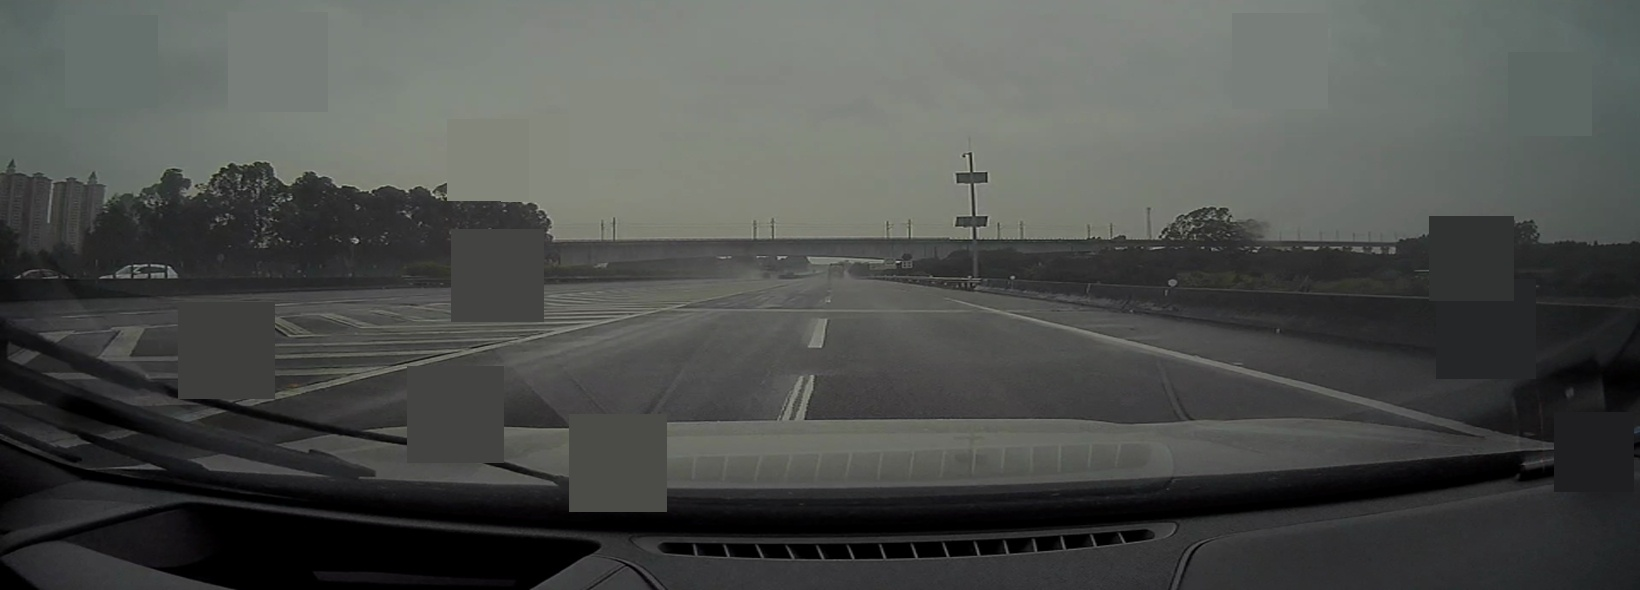
\includegraphics[width=\textwidth]{image/chap03/s4_2427000_重度遮挡.jpg}
		\caption{局部遮挡}
	\end{subfigure}
	\caption{RainLane 中典型雨天干扰形式示例}
	\label{fig:rainlane_cases}
\end{figure}


\section{本章小结}
\label{sec:summary_3}

本章围绕雨天车道线专用数据集的构建与增强展开研究。

首先，从物理机制层面分析了雨天环境中雨滴遮挡（式\ref{eq:raindrop_model}）、路面水膜镜面反射（式\ref{eq:fresnel}）以及大气散射导致的对比度退化（式\ref{eq:koschmieder}）三类主要干扰因素，并从对比度、边缘响应和结构连续性三个与检测任务直接相关的角度解释了车道线特征退化现象，为后续算法设计提供了依据。

其次，制定了多维度覆盖的真实雨天数据采集方案，并通过三级质控机制和专用标注规范（含断点续标规则），完成了约 6017 张有效样本的标注，构建了 RainLane 数据集。该数据集在降雨强度、光照条件及道路类型等维度上具有较好的覆盖性，其具体分布如表\ref{tab:dataset_split}所示。

最后，设计了包含雨纹合成（式\ref{eq:rain_synthesis}）、水膜反射模拟（式\ref{eq:reflection_aug}）、CutOut 遮挡及通用几何/光度增强的多层次数据增强流水线（算法\ref{alg:aug_pipeline}），其增强参数与强度分级与本文实际采用的增强流程保持一致。经增强处理后，样本总数扩充至 24068 张，在一定程度上缓解了极端场景样本不足的问题。本章的工作为第四章面向雨天的检测算法设计提供了直接的数据基础。
